% connecting the trees of a forest with edge e
\begin{figure}[htb]
\centering
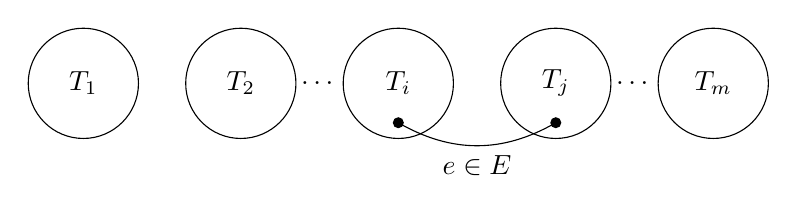
\begin{tikzpicture}
\node[] (T1) at (0,0) {$T_1$};
\node[] (T2) at (2,0) {$T_2$};
\node[] (T_dots1) at (3,0) {\ldots};
\node[] (Ti) at (4,0) {$T_i$};
\node[] (Tj) at (6,0) {$T_j$};
\node[] (T_dots2) at (7,0) {\ldots};
\node[] (Tm) at (8,0) {$T_m$};
\node[] (Ti_e) at (4,-0.5) {};
\node (Tj_e) at (6,-0.5) {};

\draw \foreach \n in {T1, T2, Ti,Tj,Tm}
{
	(\n) circle (0.7)
};

\fill (Ti_e) circle [radius=2pt];
\fill (Tj_e) circle [radius=2pt];

\path (Ti_e.center) edge [bend right] node[below] {$e \in E$} (Tj_e.center) ;

\end{tikzpicture}
\caption{Forest $F_2$ and its trees}
\end{figure}

